\documentclass[11pt,a4paper]{article}

% --- Encodage et langue ----------------------------------------------------
\usepackage[utf8]{inputenc}
\usepackage[T1]{fontenc}
\usepackage{lmodern}
\usepackage[french]{babel}
\usepackage{textcomp} % symbole euro (\texteuro / €)

% --- Mise en page ----------------------------------------------------------
\usepackage[a4paper,margin=2.4cm]{geometry}
\usepackage{microtype}
\usepackage{booktabs}
\usepackage{array}
\usepackage{graphicx}
\graphicspath{{figures/}}
\usepackage{caption}
\captionsetup{font=small,labelfont=bf}
\usepackage{xcolor}
\definecolor{bleu}{HTML}{1A3C6E}
\definecolor{grisclair}{HTML}{F4F6FA}
\usepackage{fancyhdr}
\usepackage{enumitem}
\setlist{itemsep=2pt,topsep=3pt}

% --- Liens -----------------------------------------------------------------
\usepackage[colorlinks=true,linkcolor=bleu,urlcolor=bleu,citecolor=bleu]{hyperref}

% --- Titres de section colorés ---------------------------------------------
\usepackage{titlesec}
\titleformat{\section}{\Large\bfseries\color{bleu}}{\thesection}{0.6em}{}
\titleformat{\subsection}{\large\bfseries\color{bleu!85!black}}{\thesubsection}{0.6em}{}

% --- Code ------------------------------------------------------------------
\usepackage{listings}
\lstset{
  basicstyle=\ttfamily\small,
  backgroundcolor=\color{grisclair},
  frame=single, rulecolor=\color{gray!40},
  breaklines=true, columns=fullflexible,
  keywordstyle=\color{bleu}\bfseries,
  commentstyle=\color{gray},
  showstringspaces=false,
  language=Python,
}

% --- En-tête / pied de page ------------------------------------------------
\pagestyle{fancy}
\fancyhf{}
\fancyhead[L]{\small\color{bleu}Marché de l'emploi Data en Île-de-France}
\fancyhead[R]{\small\thepage}
\renewcommand{\headrulewidth}{0.4pt}

% ===========================================================================
\begin{document}

% --- Page de titre ---------------------------------------------------------
\begin{titlepage}
\centering
\vspace*{2cm}
{\small\scshape Université Paris 1 Panthéon-Sorbonne \\ Master 1 MIAGE — Atelier IA\par}
\vspace{2.5cm}
{\color{bleu}\rule{\linewidth}{1.2pt}\par}
\vspace{0.6cm}
{\Huge\bfseries Analyse du marché de l'emploi Data\\[0.3cm] en Île-de-France\par}
\vspace{0.5cm}
{\large\itshape Collecte automatisée via l'API France Travail,\\ nettoyage, calcul et analyse\par}
\vspace{0.4cm}
{\color{bleu}\rule{\linewidth}{1.2pt}\par}
\vspace{2cm}
{\large\textbf{Question de recherche}\par}
\vspace{0.3cm}
\begin{minipage}{0.85\linewidth}\centering\itshape
« Quelles compétences Data sont les plus demandées en Île-de-France
et comment se valorisent-elles salarialement ? »
\end{minipage}
\vfill
{\large Yanis Hamitouche \quad\textbullet\quad [Nom du binôme]\par}
\vspace{0.5cm}
{\large \today\par}
\end{titlepage}

\tableofcontents
\thispagestyle{empty}
\clearpage

% ===========================================================================
\section{Introduction et contexte}

Ce dossier présente une analyse du marché de l'emploi dans les métiers de la
donnée (Data Analyst, Data Engineer, Data Scientist, Business Intelligence) en
Île-de-France, construite à partir de données collectées \emph{automatiquement}.
L'objectif est double : (i) démontrer une chaîne de traitement reproductible — de
la collecte à l'analyse — et (ii) répondre, chiffres à l'appui, à la question fil
rouge énoncée en page de titre.

La démarche suit cinq étapes, matérialisées par des scripts numérotés et
ré-exécutables : collecte (\texttt{01\_collecte.py}), nettoyage
(\texttt{02\_nettoyage.py}), calcul (\texttt{03\_calculs.py}), analyse
(\texttt{04\_analyse.ipynb}) et synthèse (le présent dossier). Chaque choix
technique est justifié ci-dessous.

% ===========================================================================
\section{Plan de récolte de données}
\label{sec:collecte}

\subsection{Comparaison des techniques de collecte}

Trois familles de techniques, vues en cours, permettent de récolter des offres
d'emploi en ligne. Nous les avons évaluées selon quatre critères déterminants
pour un travail rigoureux et reproductible.

\begin{table}[h]
\centering
\small
\begin{tabular}{>{\raggedright}p{3cm}p{4.4cm}p{4.4cm}}
\toprule
\textbf{Critère} & \textbf{API REST (France Travail)} & \textbf{Scraping job board} \\
\midrule
Légalité & Licence de réutilisation officielle & Souvent contraire aux CGU \\
Robustesse & JSON structuré et versionné & HTML fragile, casse aux refontes \\
Pertinence & Aucun rendu JS à charger & Navigateur \emph{headless} lourd \\
Reproductibilité & Requêtes paramétrées rejouables & Dépend du DOM courant \\
\bottomrule
\end{tabular}
\caption{Comparaison des approches de collecte.}
\end{table}

Conformément au principe \textbf{« API si disponible $>$ parsing HTML $>$
navigateur \emph{headless} »}, nous avons retenu l'\textbf{API REST officielle
« Offres d'emploi v2 » de France Travail} (ex-Pôle Emploi). Le \emph{scraping}
d'Indeed, LinkedIn ou Welcome to the Jungle a été écarté : il est juridiquement
risqué (CGU), techniquement fragile (le HTML change sans préavis) et superflu
puisqu'une API officielle expose exactement la donnée recherchée. Selenium /
Playwright n'auraient été qu'un dernier recours en l'absence d'API ; ici aucun
rendu JavaScript n'est à charger, donc aucun navigateur \emph{headless} n'est
nécessaire.

\subsection{Présentation de la source}

L'API expose les offres diffusées par France Travail et ses partenaires via une
ressource de recherche paginée :
\begin{center}
\texttt{GET https://api.francetravail.io/partenaire/offresdemploi/v2/offres/search}
\end{center}
Chaque offre est un objet JSON riche : identifiant, intitulé, description, dates,
lieu de travail (commune, département, coordonnées), entreprise, type de contrat,
expérience, salaire, compétences, code et libellé ROME, secteur d'activité. Cette
structure stable nous dispense de tout \emph{parsing} HTML.

\subsection{Authentification OAuth2}

L'accès repose sur \textbf{OAuth2 avec le grant \texttt{client\_credentials}} :
une authentification \emph{applicative} (sans utilisateur final), adaptée à un
traitement automatisé. Le script échange l'identifiant et le secret client contre
un jeton \emph{Bearer}.

\begin{lstlisting}
def obtenir_token(config):
    reponse = requests.post(config["token_url"], data={
        "grant_type": "client_credentials",
        "client_id": config["client_id"],
        "client_secret": config["client_secret"],
        "scope": config["scope"],
    })
    reponse.raise_for_status()
    return reponse.json()["access_token"]
\end{lstlisting}

Deux valeurs ont été \textbf{vérifiées sur la documentation Swagger} plutôt
qu'inventées :
\begin{itemize}
  \item \textbf{Endpoint token} :
  \texttt{https://entreprise.francetravail.fr/connexion/oauth2/access\_token?realm=/partenaire}
  \item \textbf{Scopes obligatoires} : \texttt{api\_offresdemploiv2 o2dsoffre}
\end{itemize}

\paragraph{Sécurité des secrets.} Les identifiants ne figurent jamais en clair :
ils résident dans un fichier \texttt{.env} exclu du dépôt (\texttt{.gitignore}),
tandis qu'un \texttt{.env.example} documente les clés attendues. C'est une bonne
pratique essentielle pour un dépôt partagé en binôme.

\subsection{Définition du périmètre}

\begin{itemize}
  \item \textbf{Géographie} : Île-de-France via le paramètre \texttt{region=11}.
  Ce choix a été préféré au filtre \texttt{departement}, \emph{limité à 5 valeurs
  par l'API} alors que l'IDF compte 8 départements. Le département reste
  récupérable dans chaque offre (champ \texttt{lieuTravail}) pour l'analyse fine.
  \item \textbf{Métiers} : recherche par mots-clés — \texttt{data analyst},
  \texttt{data engineer}, \texttt{data scientist}, \texttt{business intelligence},
  \texttt{BI} — avec un fichier brut distinct par mot-clé pour tracer l'origine de
  chaque offre.
  \item \textbf{Fenêtre temporelle} : offres créées sur les \textbf{30 derniers
  jours} (\texttt{minCreationDate} / \texttt{maxCreationDate}), soit une
  photographie récente du marché.
\end{itemize}

\subsection{Pagination et respect du quota}

L'API renvoie au plus \textbf{150 offres par appel} via le paramètre
\texttt{range=p-d}, avec les bornes imposées $p \le 3000$ et $d \le 3149$. Le
script parcourt les pages tant que le code HTTP vaut \texttt{206} (réponse
partielle) et s'arrête sur \texttt{200} (page complète) ou \texttt{204} (aucune
offre). Une pause de \texttt{0,3 s} entre les appels respecte le quota d'environ
\textbf{4 appels/seconde} par application ; les erreurs transitoires
(\texttt{429}, \texttt{5xx}) déclenchent des relances avec \emph{back-off}.

\subsection{Volumétrie obtenue}

La collecte a produit \textbf{331 offres brutes} (avant dédoublonnage), écrites en
JSON UTF-8 dans \texttt{data/raw/} — dossier traité comme \textbf{immuable} et non
versionné. Aucun mot-clé n'a atteint le plafond de l'API : la photographie du
marché sur la fenêtre considérée est donc complète.

% ===========================================================================
\section{Stratégie de nettoyage}
\label{sec:nettoyage}

Le script \texttt{02\_nettoyage.py} transforme les JSON bruts en tables propres
(\texttt{data/processed/}). Principe directeur : \texttt{data/raw/} n'est
\emph{jamais} modifié ; tout traitement est rejouable à l'identique.

\subsection{Dédoublonnage}

Une même offre peut remonter sur plusieurs mots-clés (par exemple un poste
« Data Engineer (BI) »). Le dédoublonnage par identifiant \texttt{id} ramène le
corpus de \textbf{331 à 299 offres uniques} ($-32$ doublons), évitant de
sur-pondérer les offres polyvalentes.

\subsection{Normalisation des champs}

Les objets imbriqués sont aplatis en colonnes exploitables. En particulier, le
\textbf{département} est dérivé du préfixe « \texttt{NN - VILLE} » du champ
\texttt{lieuTravail.libelle} ; l'entreprise, le type de contrat, l'expérience, le
métier ROME et le secteur sont extraits dans des colonnes dédiées, et les dates
sont typées.

\subsection{Parsing du salaire}

Le salaire est fourni en \textbf{texte libre} (\texttt{salaire.libelle}) et
n'est présent que sur une minorité d'offres. Une expression régulière extrait la
période, le minimum et le maximum des formats observés (par exemple
\emph{« Annuel de 50000.0 Euros à 55000.0 Euros sur 12 mois »}), puis
\textbf{normalise en base annuelle} selon les hypothèses suivantes, explicitées
car elles introduisent une approximation :

\begin{table}[h]
\centering\small
\begin{tabular}{lll}
\toprule
\textbf{Période} & \textbf{Facteur annuel} & \textbf{Hypothèse} \\
\midrule
Annuel & $\times 1$ & valeur déjà annuelle \\
Mensuel & $\times N$ & $N$ versements/an (12 par défaut) \\
Horaire & $\times 1820$ & temps plein 35\,h $\times$ 52 semaines \\
\bottomrule
\end{tabular}
\caption{Normalisation des salaires en base annuelle.}
\end{table}

L'hypothèse horaire est la plus fragile (sensible au temps partiel) ; elle est
donc signalée. Au final, \textbf{27\,\% des offres} disposent d'un salaire annuel
exploitable : c'est une limite assumée, quantifiée et discutée en conclusion.

\subsection{Détection des compétences}

Le champ structuré \texttt{competences[]} n'est renseigné que sur \textbf{$\sim$15\,\%}
des offres — insuffisant pour répondre à une question portant précisément sur les
compétences. Nous avons donc construit un \textbf{lexique curé de technologies
Data} (langages, bases de données, big data, cloud, BI, \emph{machine learning},
outils) et détecté leur présence par expressions régulières dans l'intitulé, la
description et les libellés de compétences. La couverture passe ainsi à
\textbf{75\,\% des offres}.

\paragraph{Justification et limites.} Ce choix méthodologique est un compromis
explicite entre exhaustivité et précision. Les motifs courts ou ambigus (par
exemple \texttt{SAS}, qui désigne aussi une forme juridique, ou \texttt{R}, lettre
isolée) sont volontairement encadrés par des frontières de mots ; un contrôle
manuel estime les faux positifs résiduels à \emph{environ 5\,\%} sur ces motifs —
acceptable au regard du gain de couverture (de 15\,\% à 75\,\%). Le résultat est
matérialisé par une table au format long \texttt{(id, competence)} qui facilite
les comptages en aval.

\subsection{Bilan de qualité des données}

\begin{table}[h]
\centering\small
\begin{tabular}{lc}
\toprule
\textbf{Indicateur} & \textbf{Valeur} \\
\midrule
Offres brutes collectées & 331 \\
Offres uniques (après dédoublonnage) & 299 \\
Départements distincts couverts & 8 \\
Entreprises distinctes & 97 \\
Compétences distinctes détectées & 53 \\
Taux de salaire annuel exploitable & 27\,\% \\
Couverture compétences (détection texte) & 75\,\% \\
\bottomrule
\end{tabular}
\caption{Synthèse de la qualité du corpus nettoyé.}
\end{table}

% ===========================================================================
\section{Calcul des indicateurs}
\label{sec:calculs}

Le script \texttt{03\_calculs.py} produit les agrégats consommés par le notebook,
de sorte que l'analyse ne recalcule rien de lourd :
\begin{itemize}
  \item \texttt{top\_competences.csv} : volume et part des offres par compétence ;
  \item \texttt{competences\_salaire.csv} : salaire annuel médian et quartiles par
  compétence, \textbf{filtré sur un effectif $\ge 5$} pour écarter les médianes
  peu fiables ;
  \item répartitions par département, type de contrat, expérience et métier ROME ;
  \item \texttt{kpi\_global.csv} : indicateurs de synthèse.
\end{itemize}

\paragraph{Choix de la médiane.} Les salaires sont résumés par la \textbf{médiane}
plutôt que la moyenne, afin de résister aux valeurs extrêmes — un salaire aberrant
à 492\,000\,\texteuro{} est en effet présent dans les données. Le seuil d'effectif
($\ge 5$) garantit que les comparaisons inter-compétences reposent sur une base
statistique minimale. \textbf{Chiffres clés} : salaire annuel médian
$\approx$~50\,000\,\texteuro{} (Q1~$\approx$~37\,k\texteuro, Q3~$\approx$~56\,k\texteuro),
69\,\% de CDI.

% ===========================================================================
\section{Analyse}
\label{sec:analyse}

L'analyse complète et interactive figure dans \texttt{notebooks/04\_analyse.ipynb}
(ré-exécutable de bout en bout). Les figures ci-dessous en synthétisent les
résultats.

\subsection{Panorama du corpus}

\begin{figure}[h]
\centering
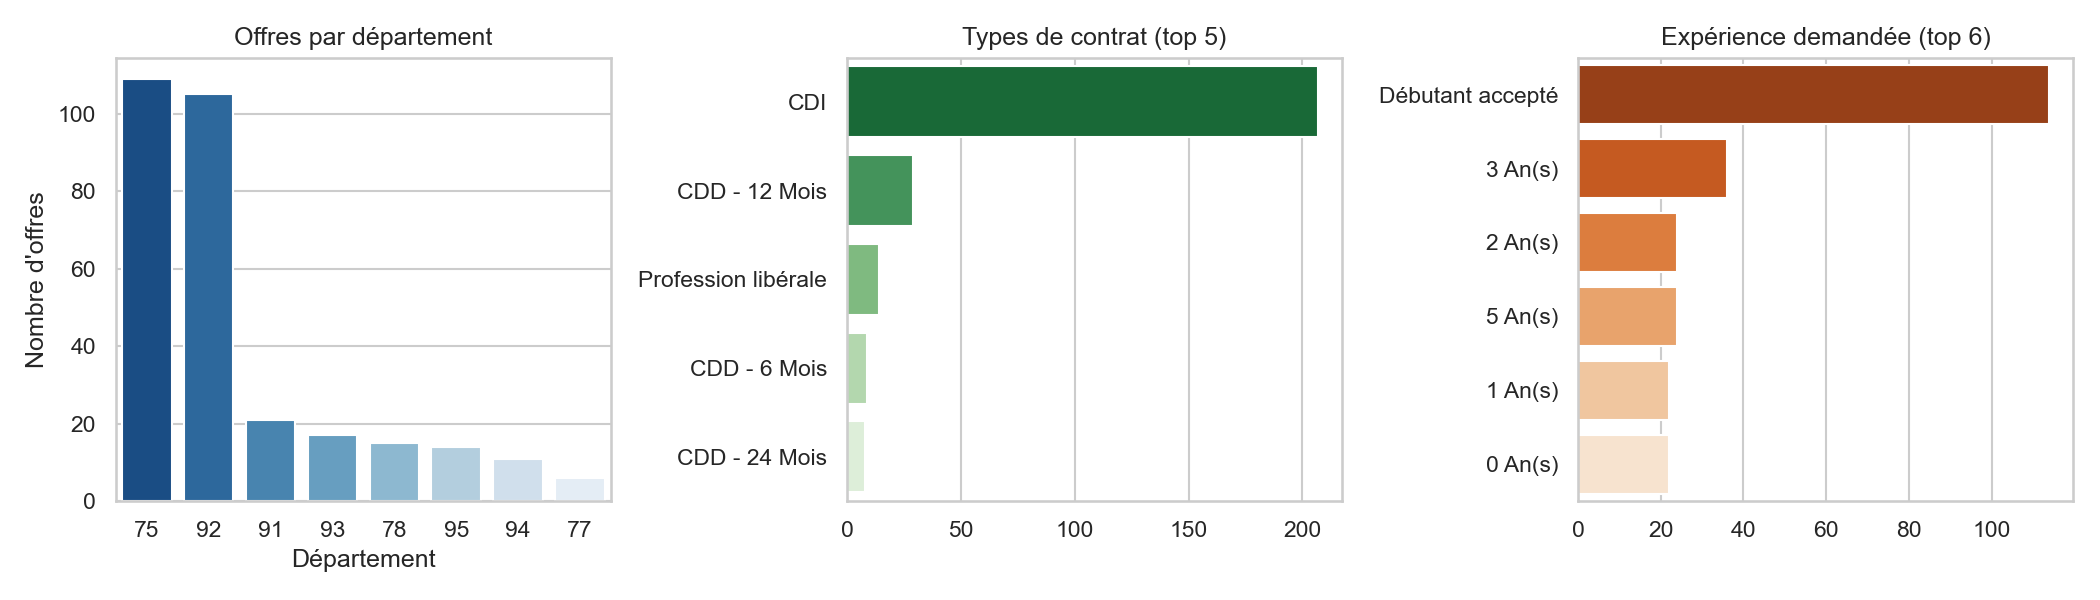
\includegraphics[width=\linewidth]{fig-panorama.png}
\caption{Répartition des offres par département, type de contrat et expérience.}
\end{figure}

L'emploi Data francilien est \textbf{fortement concentré sur Paris (75) et les
Hauts-de-Seine (92)}, qui regroupent l'essentiel des offres — reflet de la
localisation des sièges sociaux et des ESN. Le \textbf{CDI domine} nettement, et
les offres ciblent surtout des profils expérimentés.

\subsection{Compétences les plus demandées}

\begin{figure}[h]
\centering
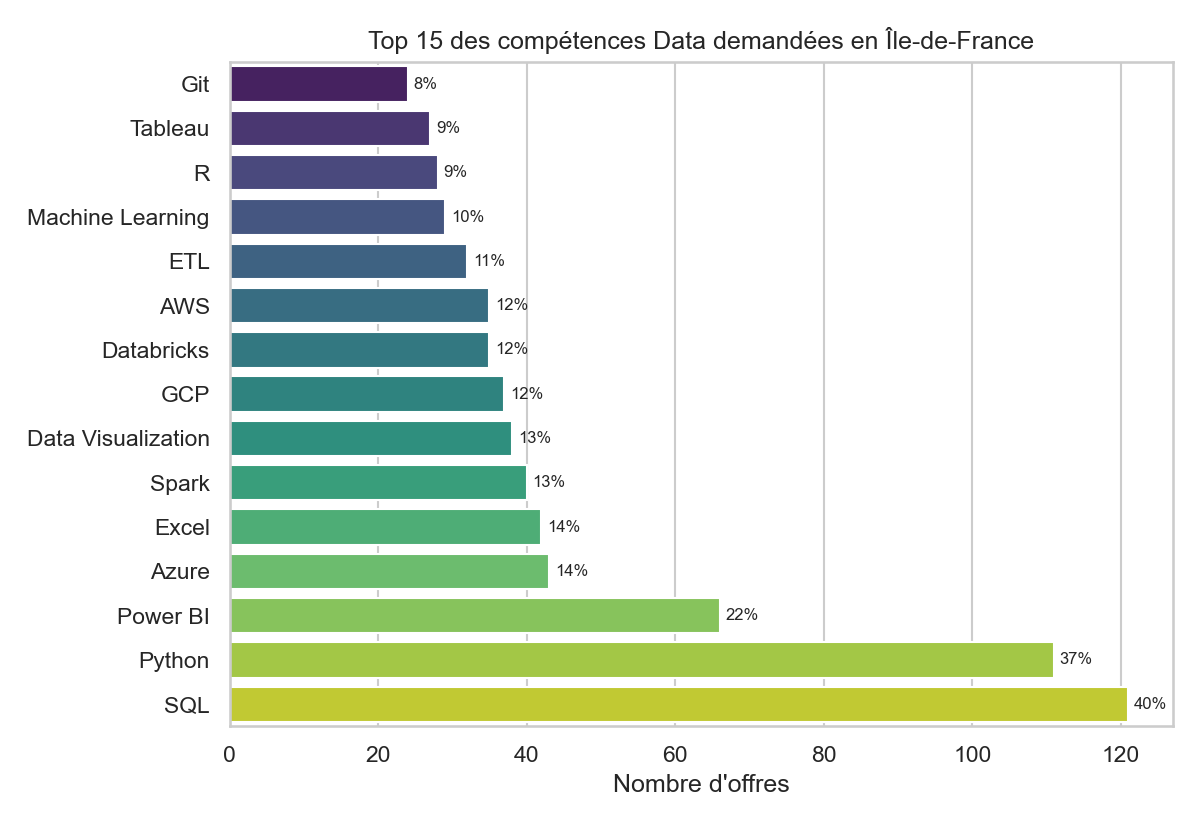
\includegraphics[width=0.92\linewidth]{fig-demande.png}
\caption{Top 15 des compétences Data demandées (part des offres en étiquette).}
\end{figure}

\textbf{SQL} et \textbf{Python} constituent le socle incontournable, présents dans
une large part des offres. Suivent la \textbf{BI / dataviz} (Power BI, Excel,
Tableau) et l'écosystème \textbf{cloud / big data} (Azure, GCP, AWS, Spark,
Databricks). La demande se structure ainsi en deux familles : un noyau analytique
et une couche d'ingénierie de la donnée.

\subsection{Valorisation salariale par compétence}

\begin{figure}[h]
\centering
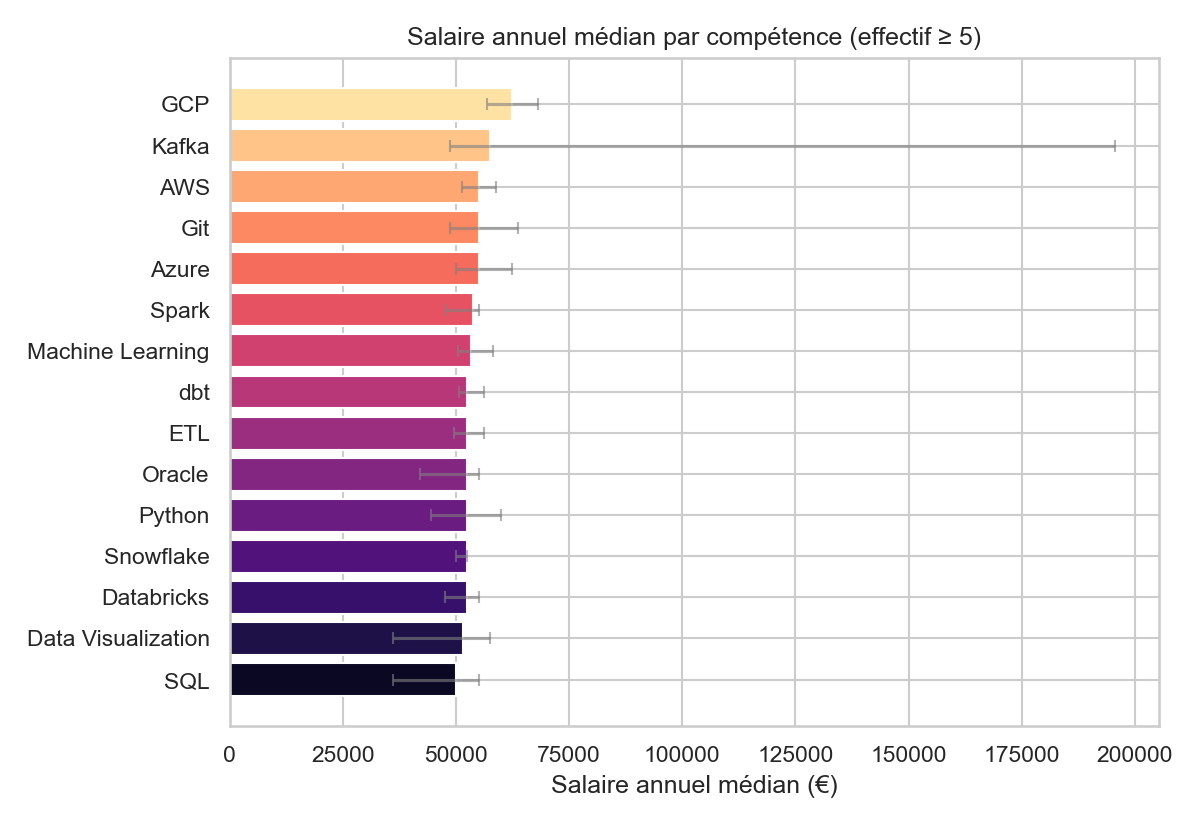
\includegraphics[width=0.92\linewidth]{fig-salaire.png}
\caption{Salaire annuel médian par compétence (effectif $\ge 5$ ; barres
d'erreur = intervalle interquartile).}
\end{figure}

Les compétences les mieux rémunérées relèvent du \textbf{cloud et du big data}
(GCP, AWS, Azure, Spark, Kafka, Databricks, Snowflake), au-dessus du socle
analytique. La maîtrise de l'\emph{infrastructure} de données se valorise donc
davantage que les seuls outils de restitution (BI).

\subsection{Synthèse : demande croisée à la valorisation}

\begin{figure}[h]
\centering
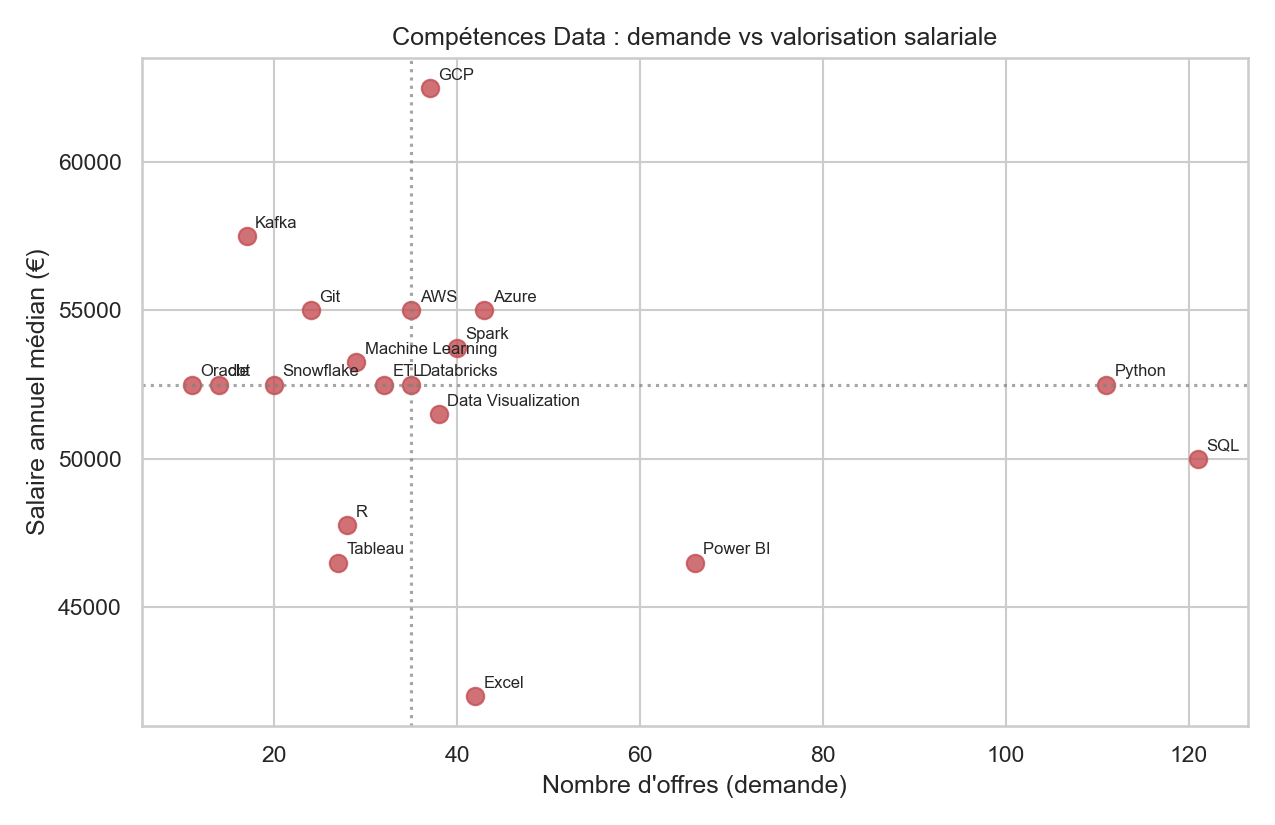
\includegraphics[width=0.9\linewidth]{fig-scatter.png}
\caption{Positionnement des compétences selon la demande (axe X) et la
valorisation salariale médiane (axe Y).}
\end{figure}

Ce croisement distingue deux profils de compétences : des compétences
\emph{socle}, très demandées mais peu différenciantes salarialement (SQL, Python),
et des compétences \emph{premium} (cloud, traitement distribué) qui tirent les
rémunérations vers le haut tout en étant moins universelles.

% ===========================================================================
\section{Conclusion}
\label{sec:conclusion}

\subsection{Réponse à la question fil rouge}

En Île-de-France, le marché Data repose sur un \textbf{socle SQL + Python}
quasi universel, complété par la \textbf{BI} et, de plus en plus, par
l'\textbf{ingénierie de la donnée dans le cloud}. Côté rémunération,
\textbf{ce sont les compétences cloud et big data qui se valorisent le mieux} :
SQL et Python sont nécessaires mais peu distinctifs, tandis qu'un profil
\emph{Data Engineer} maîtrisant un cloud (Azure / GCP / AWS) et le traitement
distribué (Spark / Databricks) se situe en haut de l'échelle salariale, devant le
\emph{Data Analyst} BI seul.

\subsection{Limites et biais}

\begin{itemize}
  \item \textbf{Biais de source} : les offres France Travail ne représentent
  \emph{pas} le marché total. De nombreux postes cadres sont diffusés via d'autres
  canaux (LinkedIn, cabinets, cooptation) ; le haut du marché est probablement
  sous-estimé.
  \item \textbf{Couverture salariale} : seules 27\,\% des offres affichent un
  salaire exploitable — les médianes par compétence, fondées sur de petits
  effectifs (d'où le seuil $\ge 5$), sont à lire comme des ordres de grandeur.
  \item \textbf{Détection lexicale} : quelques faux positifs résiduels
  ($\sim$5\,\% sur les motifs courts), et un lexique curé mais non exhaustif.
  \item \textbf{Fenêtre temporelle} : une collecte sur 30 jours est une
  photographie, non une tendance ; elle peut refléter une saisonnalité.
\end{itemize}

\subsection{Pistes d'amélioration}

Élargir la fenêtre temporelle et croiser plusieurs sources (autres API, données
INSEE / DARES) ; enrichir le lexique et fiabiliser la détection par des techniques
de TAL (NLP) ; suivre l'évolution dans le temps pour passer d'une photographie à
une véritable analyse de tendance.

% ===========================================================================
\appendix
\section{Reproductibilité}

Le dépôt est organisé selon une structure standard (\texttt{src/},
\texttt{data/raw}, \texttt{data/processed}, \texttt{notebooks/},
\texttt{rapport/}). Après installation des dépendances
(\texttt{pip install -r requirements.txt}) et configuration du fichier
\texttt{.env}, le pipeline s'exécute dans l'ordre :

\begin{lstlisting}[language=bash]
python src/01_collecte.py     # collecte API -> data/raw/
python src/02_nettoyage.py    # nettoyage   -> data/processed/
python src/03_calculs.py      # KPI / agrégats
jupyter notebook notebooks/04_analyse.ipynb
\end{lstlisting}

Les figures de ce dossier sont régénérées par
\texttt{python rapport/build\_figures.py}.

\end{document}
